\documentclass[a11paper, 11pt]{article}

\usepackage{libs/document}
\usepackage{libs/titlepage}
\usepackage{listings}
\usepackage{graphicx}
\usepackage{array}
% \usepackage{minted}
\usepackage{multicol}
\usepackage[T1]{fontenc}
\usepackage[french]{babel}

% \addbibresource{refs/bibliography.bib}
% \nofiles


\lstset{%
        inputencoding=utf8,
        extendedchars=true,
        basicstyle=\footnotesize\ttfamily,
        showstringspaces=false,
        showspaces=false,
        % numbers=left,
        % numberstyle=\footnotesize,
        numbersep=9pt,
        tabsize=2,
        breaklines=true,
        showtabs=false,
        captionpos=b,
        literate=%
        {é}{{\'{e}}}1
        {è}{{\`{e}}}1
        {ê}{{\^{e}}}1
        {ë}{{\¨{e}}}1
        {É}{{\'{E}}}1
        {Ê}{{\^{E}}}1
        {û}{{\^{u}}}1
        {ù}{{\`{u}}}1
        {ú}{{\'{u}}}1
        {â}{{\^{a}}}1
        {à}{{\`{a}}}1
        {À}{{\`{A}}}1
        {á}{{\'{a}}}1
        {ã}{{\~{a}}}1
        {Á}{{\'{A}}}1
        {Â}{{\^{A}}}1
        {Ã}{{\~{A}}}1
        {ç}{{\c{c}}}1
        {Ç}{{\c{C}}}1
        {õ}{{\~{o}}}1
        {ó}{{\'{o}}}1
        {ô}{{\^{o}}}1
        {Õ}{{\~{O}}}1
        {Ó}{{\'{O}}}1
        {Ô}{{\^{O}}}1
        {î}{{\^{i}}}1
        {Î}{{\^{I}}}1
        {í}{{\'{i}}}1
        {Í}{{\~{Í}}}1
}
\renewcommand\lstlistingname{Algorithme}

% \institution{Université de Sherbrooke}
% \faculty{Faculté de génie}
% \department{Département de génie électrique et de génie informatique}
\title{Rapport d'APP}
\classnb{APP4}
\class{Atelier de programmation}
\author{
  \addtolength{\tabcolsep}{-0.4em}
  \begin{tabular}{rcl} % Ajouter des auteurs au besoin
  Benjamin Chaussé     & -- & chab1704 \\
  Guillaume Malgorn    & -- & malg1503 \\
  \end{tabular}
}
\teacher{Eugène Morin} % TODO: Est-ce le bon prof pour le rapport?
% \location{Sherbrooke}
% \date{\today}

\begin{document}
\maketitle
% \tableofcontents
\newpage


% PSEUDOCODE FONCTION pgm_lire
\begin{lstlisting}[caption=Pseudocode de la fonction findChar]
FONCTION pgm_lire ( nom_fichier[], matrice[MAX_HAUTEUR][MAX_LARGEUR], *p_lignes, *p_colonnes, *p_maxval,  MetaData *p_metadonnees) : OK
  // nom_fichier : non du fichier contenant les métadonnées
  // matrice [MAX_HAUTEUR][MAX_LARGEUR] : matrice contenant les métadonnées du fichier
  // *p_lignes : pointeur utilisé pour obtenir la résolution de l'image
  // *p_colonnes : pointeur utilisé pour obtenir la résolution de l'image
  // *p_maxval : pointeur vers MAX_VAlEUR qui est de 65535
  // MetaData : structure définis dans le fichier bibliothèque_image.h
  // *p_metadonnes : pointeur

DÉBUT
  // txt [145] (chaine de caractère)
  // firstChar (caractère) := {0}
  // filetype (entier) := 0
  // tonedepth (entier) := 0
  // readline [MAX_VALEUR] (chaine de caractère) := {0}
  // metadataAuthor [32] (chaine de caractère) := {0}
  // metadataDate [11] (chaine de caractère) := {0}
  // metadataLocation [32] (chaine de caractère) := {0}
  // metaErrs [3] (chaine d'entier) : Permet de savoir si il y a une erreur dans metadataAuthor, metadataDate, metadataLocation

  Écrire "Opening the file..." à l'écran
  FICHIER *fp := OUVERTURE(nom_fichier, LECTURE)
  SI !fp ALORS
    Ecrire "Could not open the file. Does the file exist ?" à l'écran
    Retourner ERREUR_FICHIER
  SINON
    Ecrire "Succesfully opened file." à l'écran

  Ecrire "Looking for metadata information..." à l'écran
  firstChar := fgetc(fp)
  SI firstChar == '#' ALORS
  Lire l'auteur, la date et la localisation dans le fichier fp à l'écran et envoyer dans metadataAuthor, metadataDate, metadataLocation
  metaErrs[0] := (strlen(metadataAuthor) == 0) ? 1 : 0
  metaErrs[1] := (strlen(metadataDate) == 0) ? 1 : 0
  metaErrs[2] := (strlen(metadataLocation) == 0) ? 1 : 0

  Ecrire "Metadata error array -> ", metaErrs[0], metaErrs[0], metaErrs[0] à l'écran
  Ecrire "Detected metadata contents", "Author : ", metadataAuthor, "Date : ", metadataDate, "Location : ", metadataLocation à l'écran

  SI metaErrs[0] + metaErrs[1] + metaErrs[2] > 0 ALORS
    Ecrire "Warning : One or more metadata fields could not be read properly." à l'écran
  SINON
    Ecrire "Successfully loaded metadata information" à l'écran

    COPIE metadataAuthor dans auteur de la structure MetaData
    COPIE metadataDate dans dateCreation de la structure MetaData
    COPIE metadataLocation dans lieuCreation de la structure MetaData

    Ecrire "content of metadat struct", "Author :", auteur, "Date : ", dateCreation, "Location :", lieuCreation à l'écran
    SINON
    Ecrire "No metadata information present." à l'écran

  Ecrire "verifying file format..." à l'écran
  Lire le type de l'image dans le fichier et le mettre dans filetype
  Ecrire "Detected filetype is", filetype à l'écran
  SI filetype != 2 ALORS
    Ecrire "Given file does not have a pgm filetype." à l'écran
    Retourner ERREUR_FORMAT
  SINON
    Ecrire "File format is pgm (P2) as required" à l'écran

  Ecrire "Verifying image dimensions..." à l'écran
  Lire les dimensions à l'écran et les envoyers dans p_colonnes et p_lignes
  Ecrire "Image dimensions", "Height : ", *p_lignes, "Widht : ", *p_colonnes à l'écran
    SI *p_lignes > MAX_HAUTEUR OU *p_colonnes > MAX_LARGEUR ALORS
    Ecrire "Image height and/or widht exceeds maximum value" à l'écran
    Retourner ERREUR_TAILLE
  SINON
    Ecrire "Found that image resolution is ", *p_colonnes, " x ", *p_lignes

  Ecrire "Verifying image tone depth" à l'écran
  Lire la profondeur de tonalité à l'écran et l'envoyer dans tonedepth
  Ecrire "Read a tone depth value of ", tonedepth à l'écran
  SI tonedepth > MAX_VALEUR ALORS
    Ecrire "Tone depth resolution surpasses what the spec allows" à l'écran
    Retourner ERREUR_FORMAT
  SINON
    Ecrire "Tone depth is set to ", tonedepth à l'écran

  Ecrire "Reading pixel data from file..." à l'écran
  POUR h = 0 À *p_lignes
    h := h + 1
  POUR w = 0 À *p_colonnes
    w := w + 1
  SI Lire matrice[h][w] dans le fichier fp à l'écran ALORS
    Ecrire "There was insuficient pixel data in the file" à l'écran
    Rtourner ERREUR_TAILLE
  SINON
    pixelcount := pixelcount + 1
  Ecrire "Succesfully loaded the image into the matrix" à l'écran
  Fermer fichier fp
  Retourner OK

FIN
\end{lstlisting}

\begin{figure}
  \centering
  \caption{Diagrame UML de la fonction pgm\_extraire}
  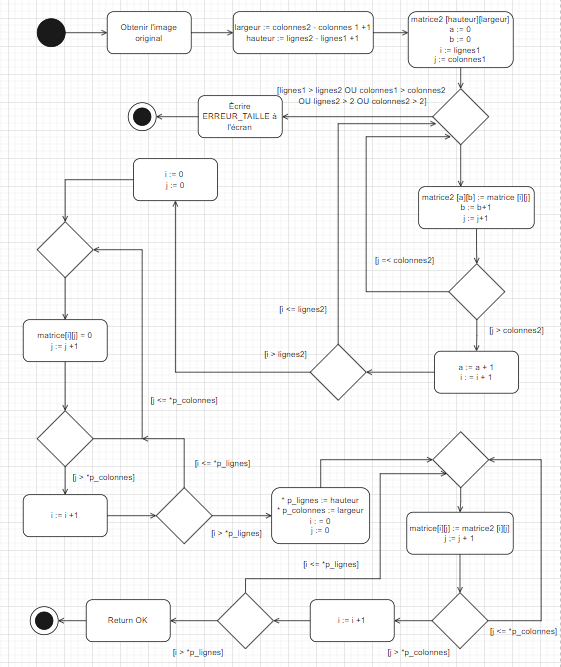
\includegraphics[width=\textwidth]{figures/diagram.png}
\end{figure}


\end{document}
